\documentclass[11pt,compress,t,notes=noshow, aspectratio=169, xcolor=table]{beamer}

\usepackage{../../style/lmu-lecture}
% Defines macros and environments
% This file is included in slides and exercises

% Rarely used fontstyle for R packages, used only in 
% - forests/slides-forests-benchmark.tex
% - exercises/single-exercises/methods_l_1.Rnw
% - slides/cart/attic/slides_extra_trees.Rnw
\newcommand{\pkg}[1]{{\fontseries{b}\selectfont #1}}

% Spacing helpers, used often (mostly in exercises for \dlz)
\newcommand{\lz}{\vspace{0.5cm}} % vertical space (used often in slides)
\newcommand{\dlz}{\vspace{1cm}}  % double vertical space (used often in exercises, never in slides)
\newcommand{\oneliner}[1] % Oneliner for important statements, used e.g. in iml, algods
{\begin{block}{}\begin{center}\begin{Large}#1\end{Large}\end{center}\end{block}}

% Don't know if this is used or needed, remove?
% textcolor that works in mathmode
% https://tex.stackexchange.com/a/261480
% Used e.g. in forests/slides-forests-bagging.tex
% [...] \textcolor{blue}{\tfrac{1}{M}\sum^M_{m} [...]
% \makeatletter
% \renewcommand*{\@textcolor}[3]{%
%   \protect\leavevmode
%   \begingroup
%     \color#1{#2}#3%
%   \endgroup
% }
% \makeatother


\title{Interpretable Machine Learning}
% \author{LMU}
%\institute{\href{https://compstat-lmu.github.io/lecture_iml/}{compstat-lmu.github.io/lecture\_iml}}
\date{}

\begin{document}

% Set style/preamble.Rnw as parent.

% Load all R packages and set up knitr

% This file loads R packages, configures knitr options and sets preamble.Rnw as 
% parent file
% IF YOU MODIFY THIS, PLZ ALSO MODIFY setup.Rmd ACCORDINGLY...

% Defines macros and environments
 \newcommand{\titlefigure}{figure/lime.png}
\newcommand{\learninggoals}{
\item Understand motivation for local explanations 
\item Develop an intuition for possible use-cases
\item Know characteristics of local explanation methods}

\lecturechapter{Introduction to Local Explanations}
\lecture{Interpretable Machine Learning}

% ------------------------------------------------------------------------------

\begin{frame}[t]{Methodological Motivation}

% Marius: We cannot write such stuff if we want to stay flexible how to combine chunks
%Except for Shapley values and ICE curves, we focused so far mostly on global explanation methods that explain global model behavior (e.g. PDP, PFI, etc.). However, there are also many methods that explain the \textbf{local} behavior of a model.

	\begin{itemize}
	    \item Purpose of local explanations:
	    \begin{itemize}
	        \item Insight into the driving factors for a \textbf{particular prediction/decision}
	        \item Understand ML model decisions in a \textbf{local neighborhood} of a given input\\ (e.g., feature vector)
	    \end{itemize}
	    \medskip
	    \pause
		\item Local Methods can address questions such as: 
		\begin{itemize}
		    \item \textbf{Why} did the model decide to predict $\yh$ for input $\xv$?
		    \item \textbf{How} does the model behave for observations similar to $\xv$?
		    \item \textbf{What if} some features of $\xv$ had different values?
		    \item  \textbf{Where} (in which regions in $\Xspace$) does the model fail?
		\end{itemize}  
	\end{itemize}
\end{frame}

\begin{frame}[t]{Social Motivation}

%All these questions can indeed be relevant for the ML modeler. However, unlike in global methods that require expert ML understanding or even domain knowledge, many local methods aim to provide explanations also for laypersons. 
	\begin{itemize}
		\item Explanations for laypersons should be tailored to the \textbf{explainee}\\ % (who receives the explanation)\\ %(i.e., the person receiving the explanation)
		%\pause
		$\leadsto$ \textbf{case specific}, \textbf{human-intelligible}, and \textbf{faithful} to the explained mechanism
		\pause
		\item If algorithms make decisions in \textbf{socially/safety critical domains}, end users have a justified interest in receiving explanations
		\pause
		\item Local explanations cannot only increase \textbf{user trust}, but also help to detect \textbf{critical local biases} in algorithmic decision making
		\pause
		\item European citizens have the legally binding \textbf{right to explanation} as given in the General Data Protection Regulation (GDPR) and the AI Act
		\begin{itemize}
		    \item[$\leadsto$] Instead of explaining the entire (complex) model (with potential market secrets), explanations in a case-by-case usage are more reasonable
		\end{itemize}

	\end{itemize}
\end{frame}


\begin{frame}[t]{GDPR \& AI Act: The Right to Explanation}

``The data subject should have the right not to be subject to a decision
    %, which may include a measure, evaluating personal aspects relating to him or her which is 
    [...] based solely on automated processing [...],
    %and which produces legal effects concerning him or her or similarly significantly affects him or her, 
    such as automatic refusal of an online credit application or e-recruiting practices without any human intervention.

$[\ldots]$

In any case, such processing should be subject to suitable safeguards, which should include [...]
%specific information to the data subject and 
the \textbf{right to obtain} [...]
%human intervention, to express his or her point of view, to obtain 
\textbf{an explanation of the decision reached after such assessment and to challenge the decision}.''
\hfill \citebutton{Recital 71, GDPR, 2016}{https://gdpr-text.com/read/recital-71}

\medskip

``Any affected person [...]
%subject to a decision which is taken by the deployer on the basis of the output from a high-risk AI system listed in Annex III, with the exception of systems listed under point 2 thereof, and which produces legal effects or similarly significantly affects that person in a way that they consider to have an adverse impact on their health, safety or fundamental rights 
shall have the right to obtain from the deployer clear and meaningful explanations of the role of the AI system in the decision-making procedure and the main elements of the decision taken.''
\hfill \citebutton{Art. 86, AI Act, 2021}{https://www.artificial-intelligence-act.com/Artificial_Intelligence_Act_Article_86.html}
\end{frame}


\begin{frame}[t]{Example: Husky or Wolf?}
	\begin{itemize}
		\item We trained a model to predict if an image shows a wolf or a husky 
		\item Below predictions on six test images are given 
		\item Do you trust our predictor? 
	\end{itemize}
	
	\begin{columns}[T, onlytextwidth]
	
	\begin{column}{0.45\textwidth}
	    \centering
    	%\begin{center}
    		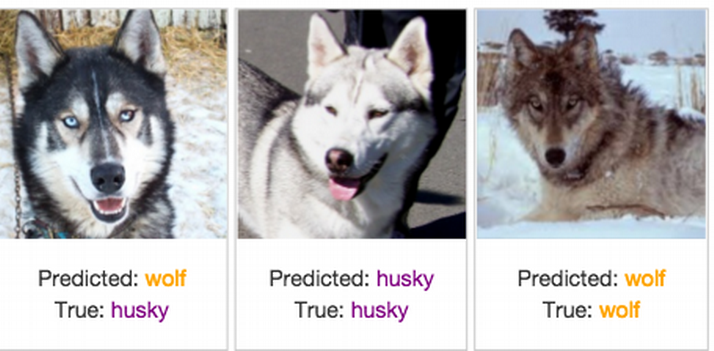
\includegraphics[width=\textwidth]{figure/lime-wolfhusky.png}\\
    		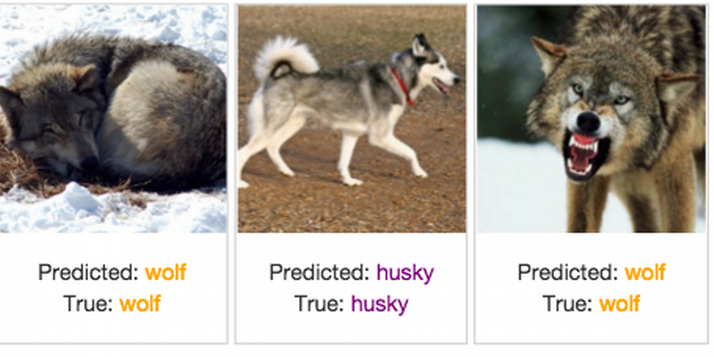
\includegraphics[width=\textwidth]{figure/lime-wolfhusky2.png}\\
    		{\textbf{Source:} [\href{http://www.facweb.iitkgp.ac.in/~niloy/COURSE/Spring2018/IntelligentSystem/PPT_2018/why_should_i_trust_ppt.pdf}{Sameer Singh 2018}]}
    	%\end{center}
	    
	\end{column}
	
	\begin{column}{0.55\textwidth}
	    
	\begin{itemize}
		\item Sometimes the ML model is wrong
		\item Can you guess the pattern the ML model learned to identify a wolf?
	\end{itemize}
	    
	\end{column}
	    
	\end{columns}

\end{frame}


\begin{frame}[t]{Example: Husky or Wolf? Using LIME}
	\begin{itemize}
		\item Local explanations highlight the parts of an image which led to the prediction\\
        $\leadsto$ our predictor is actually a snow detector 
	\end{itemize}
    
	\begin{center}
		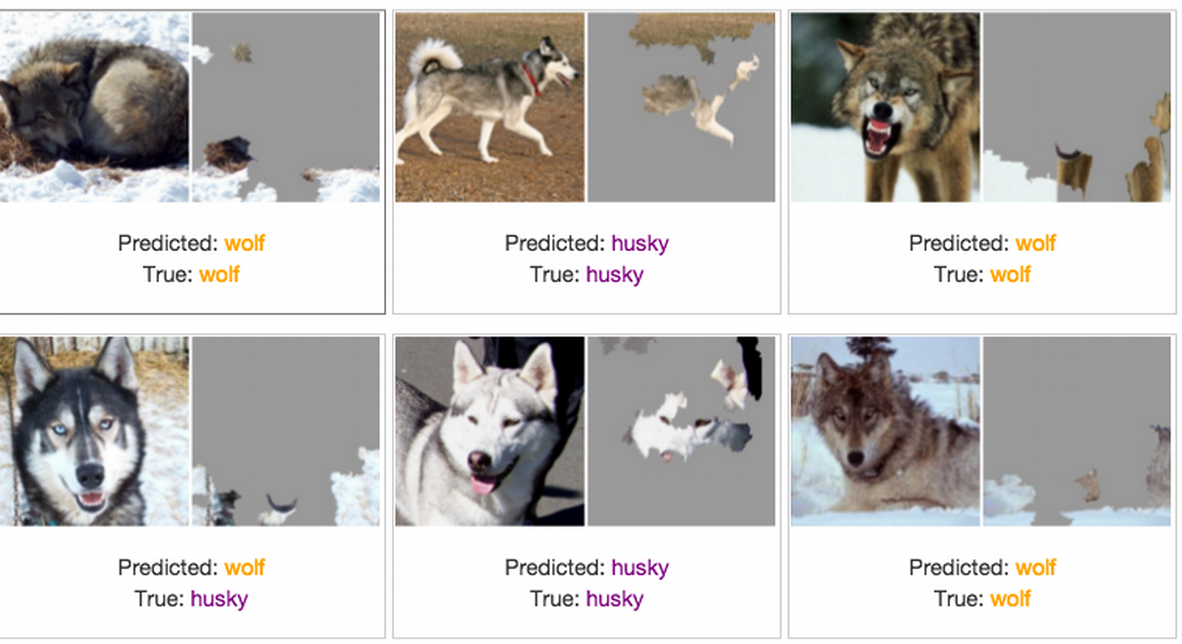
\includegraphics[width=0.9\textwidth]{figure/lime-wolfhusky3.png}\\
		{\textbf{Source:} [\href{http://www.facweb.iitkgp.ac.in/~niloy/COURSE/Spring2018/IntelligentSystem/PPT_2018/why_should_i_trust_ppt.pdf}{Sameer Singh 2018}]}
	\end{center}







\end{frame}


\begin{frame}{Example: Loan Application}

\begin{columns}[c, totalwidth=\textwidth]
    
    \begin{column}{0.45\textwidth}
        	\begin{center}
		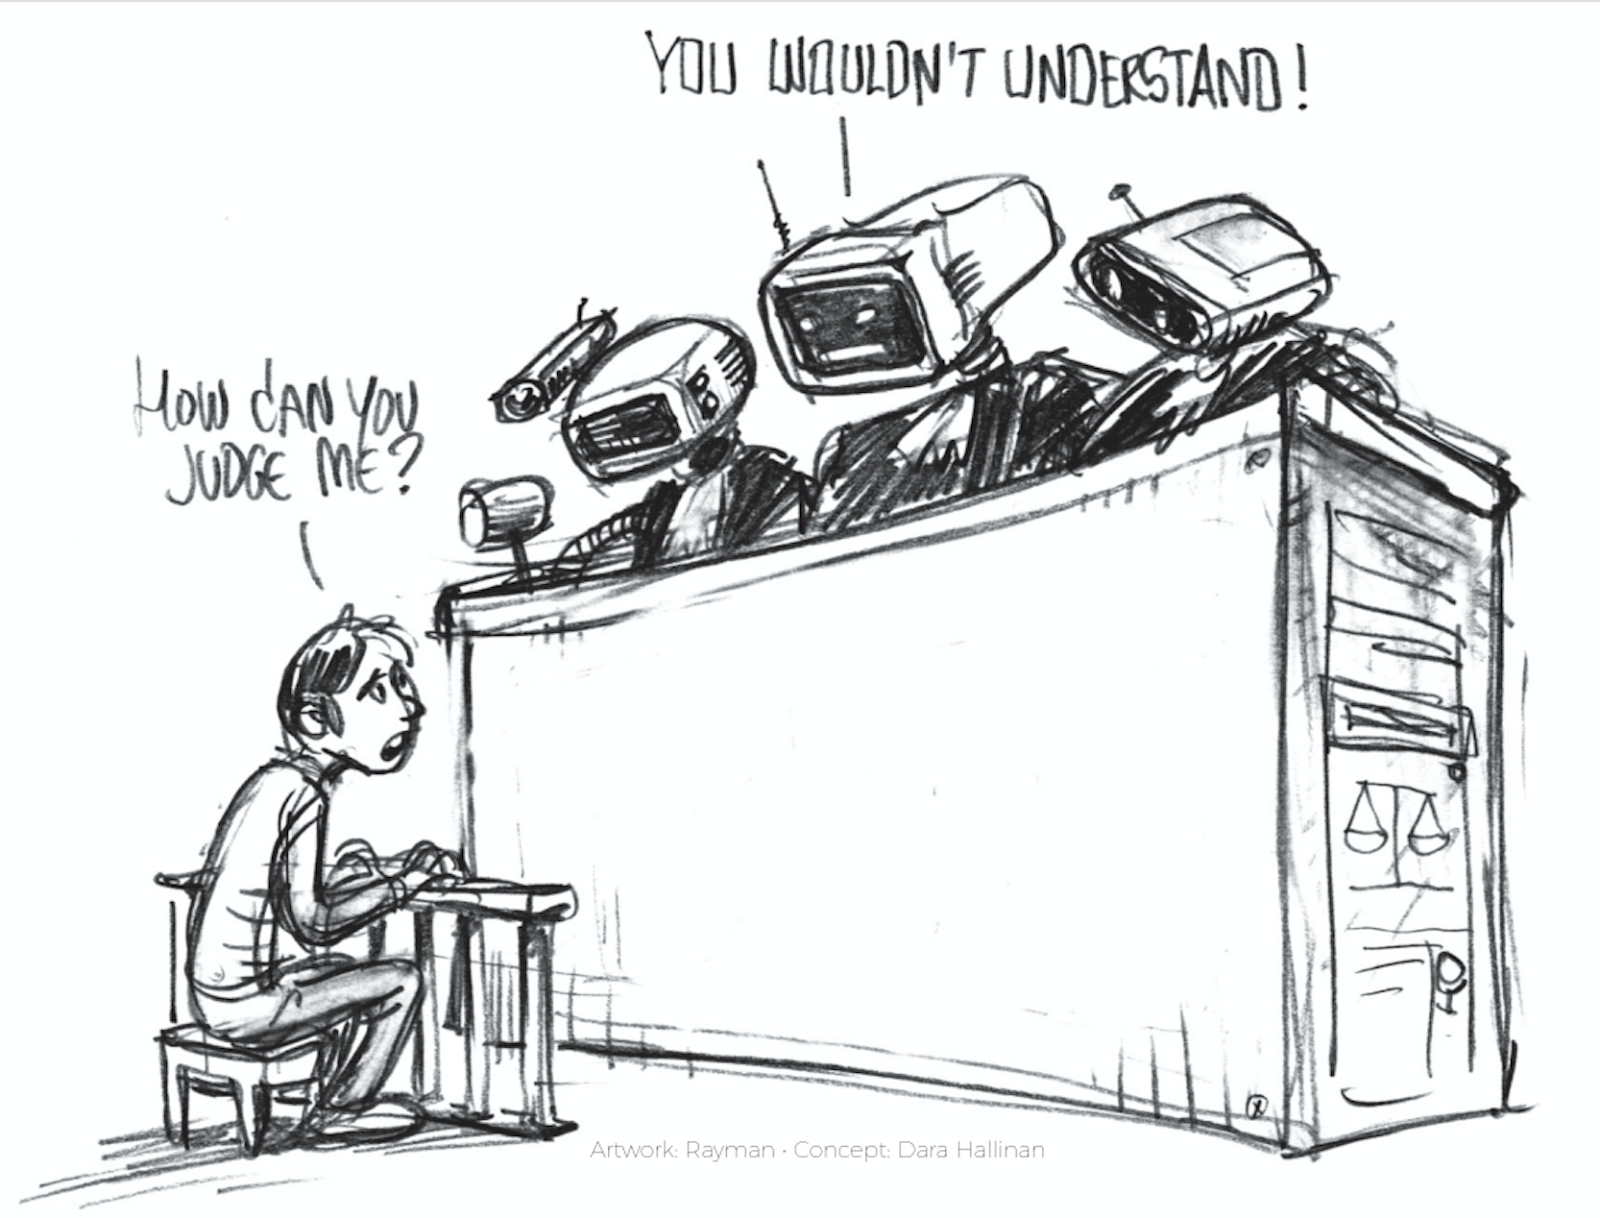
\includegraphics[width=1\textwidth]{figure/IntroJudge.png}\\
		{\textbf{Source:} [\href{https://www.elte.hu/content/trendfordulo-az-mi-fejlesztesekben.t.19025}{https://www.elte.hu}]}
	\end{center}
	
	\end{column}
	
	\begin{column}{0.55\textwidth}
	
    	\begin{itemize}
    	    \item<1-> Imagine: You apply for a loan at an online bank and are immediately rejected without reasons
    	    %Imagine: You are applying at a bank's online portal for a loan and your application gets immediately rejected without reasons
    	    \item<2-> Bank could e.g. provide a counterfactual explanation using local explanation methods:
    	    \begin{itemize}
    	        \item[] ``If you were older than 21, your loan application would have been accepted."
    	    \end{itemize}
    	    \item<3->[$\leadsto$] helps to understand the decision and to take actions for recourse (if req.)
    	\end{itemize}
    	
    \end{column}
\end{columns}

\end{frame}



\begin{frame}[t]{Example: Stop or Right-of-Way?}

\begin{columns}[c, totalwidth=\textwidth]

	\begin{column}{0.55\textwidth}
	\begin{itemize}
	    \item Imagine: 
	        \begin{itemize}
	            \item You work at a car company that develops image classifiers for autonomous driving
	            \item You show your model the following image (an adversarial example)
	            \pause
	            \item Classifier is $99\%$ sure it describes a right-of-way sign
	        \end{itemize}  
	    \item Would you entrust other peoples lives into the hands of this software?
	\end{itemize}
	
	 \end{column}
	
	\begin{column}{0.45\textwidth}

	\begin{center}
		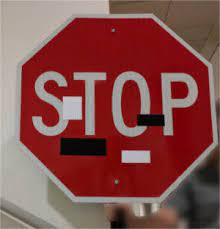
\includegraphics[width=0.7\textwidth]{figure/IntroStop.jpg}\\
		{\textbf{Source:} [\href{https://arxiv.org/abs/1707.08945}{Eykholt et. al 2018}]}
	\end{center}

     \end{column}

\end{columns}

\end{frame}

\begin{frame}[t]{Characteristics of Local Explanations}
	\begin{itemize}[<+->]
		\item \textbf{Explanation scope:} Specific prediction, local environment
		\item \textbf{Model classes:} Model-agnostic by definition, model-specific for computational reasons\\
		$\leadsto$ very popular also for deep learning models
		\item \textbf{Audience:} ML modelers and laypersons
		\item \textbf{Data types:} Often agnostic, including tabular, image, text and audio data
		\item \textbf{Methods:} Many, most prominent are counterfactual explanations, shapley values, local interpretable model-agnostic explanations (LIME), adversarial examples, single ICE curve%, anchors
		%\footnote{For Shapley values and ICE curves see other lectures}
		\item \textbf{Special:} Due to audience, strong interactions with social sciences and strong connections to cognitive science and neurosciences due to data types
	\end{itemize}
\end{frame}

% \begin{frame}{Recap: ICE Curve}
% 		\begin{itemize}
% 		\item Visualize how the model prediction $\fh(\xv)$ of a individual observation $\xv$ change by varying the feature values of one or two features while keeping all other features fixed. 
% 		\item Warning: Careful interpretation for highly correlated features or feature regions with a few observations. 
% 	\end{itemize}
% \vspace{0.5cm}
% \begin{columns}[totalwidth=\textwidth]
% 	\begin{column}{0.47\textwidth}
% 		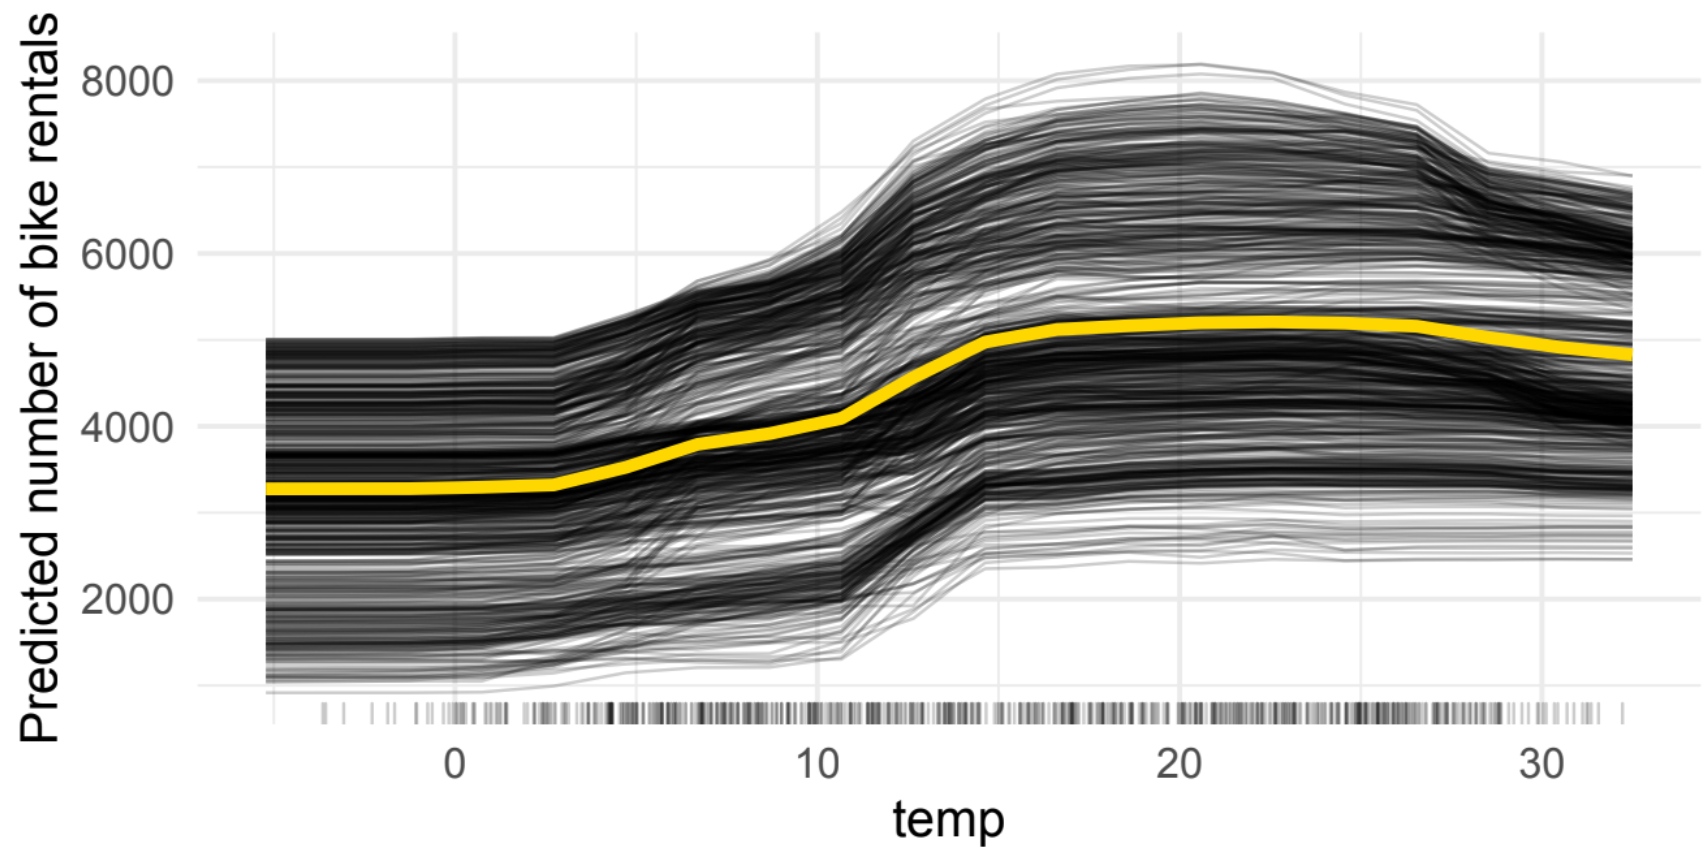
\includegraphics[width=1\textwidth]{figure/bike-sharing-dataset01.png}
% 	\end{column}
% 	\begin{column}{0.47\textwidth}
% 		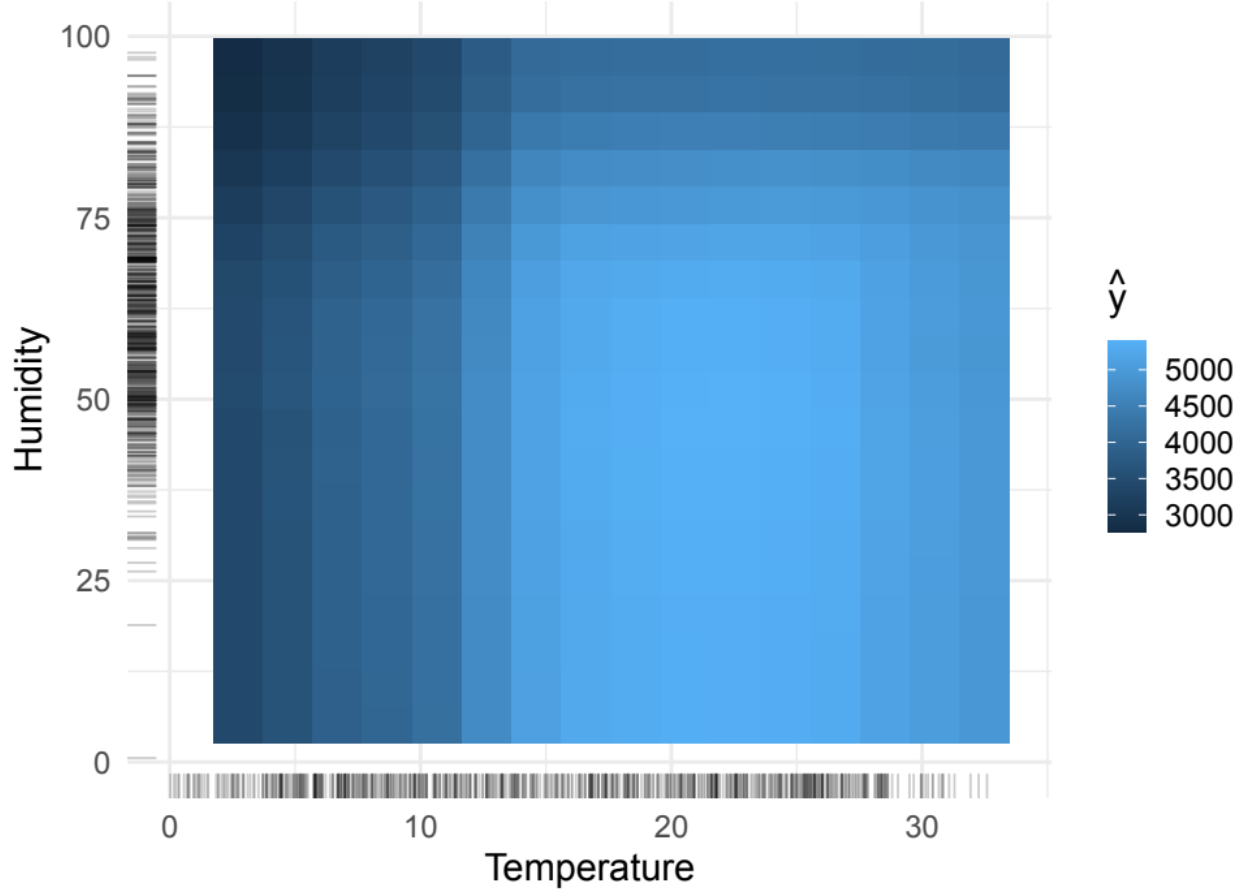
\includegraphics[width=1\textwidth]{figure/bike-sharing-dataset02.png}
% 	\end{column}
% \end{columns}
% \end{frame}

% \begin{frame}{Recap: Shapley Values}
% 	\begin{itemize}
% 		\item Shapley values were original proposed in game theory.
% 		\item They are a local explanation method because they tell us how each feature $x_j$ contributes to the overall prediction $\fh(\xv)$ of a specific observation $\xv$. 
% 	\end{itemize}
% \vspace{0.5cm}
% \begin{center}
% 	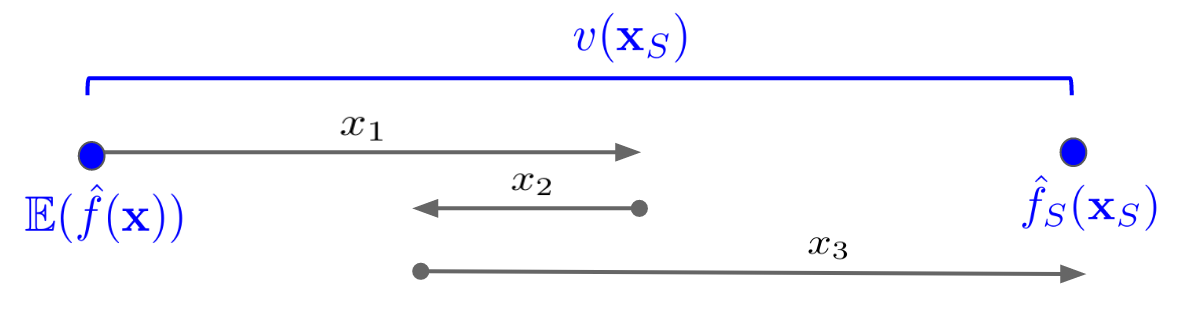
\includegraphics[width=0.8\textwidth]{figure/shapley_valuefct}
% \end{center}
% \end{frame}

\begin{frame}{Credit Dataset}

	\begin{itemize}
		\item We illustrate local explanation methods on the German credit data 
		\citebutton{see Kaggle}{https://www.kaggle.com/uciml/german-credit}
		\item 522 complete observations, 9 features containing credit and customer information
		\item Binary target ``risk'' indicates if a customer has a `good' or `bad' credit risk
		\item We merged categories with few observations 
	\end{itemize}
		\begin{center}
			\footnotesize
			\begin{tabular}{ccc}
				\toprule
				name & type & range\\
				\midrule
				age & numeric & [19, 75]\\
				sex & factor & \{male, female\}\\
				job & factor & \{0, 1, 2, 3\}\\
				housing & factor & \{free, own, rent\}\\
				saving.accounts & factor & \{little, moderate, rich\}\\
				checking.accounts & factor & \{little, moderate, rich\}\\
				credit.amount & numeric & [276, 18424]\\
				duration & numeric &  [6, 72]\\
				purpose & numeric &  \{others, car, furniture, radio/TV\}\\
				risk & factor & \{good, bad\}\\
				\bottomrule
			\end{tabular}
		\end{center}
\end{frame}

\endlecture
\end{document}
